\section{Runtime System}\label{sec:runtime-system}
The runtime system of Parallel.es consists of two parts: The slaves running in background threads executing the tasks and the public API in the main thread that forms the facade and acts as the master for the slaves. Applications are using the facade provided by the master to run functions in a background thread. The master is responsible for spawning the slaves and distributing the work onto these. It, therefore, uses a thread pool that manages the created slave instances and queues tasks if no idle slave is available. The default thread pool uses a FIFO queue and the number of slaves is limited to the number of logical processors provided by the hardware\footnote{The number of logical processors can be determined using \javascriptinline/navigator.hardwareConcurrency/. The implementation assumes the hardware has four logical processors if the API is not supported by the used browser.}. The next section describes how the runtime system processes a single task. 

\subsection{Task Roundtrip}
The steps needed to process a single task are shown in \cref{fig:runtime-system}. The application passes the task function together with the arguments to the facade that acts as the master (1). The created task is queued in the thread pool and executed on the first slave that gets available. The master transmits the serialized representation of the function call --- consisting of a unique id identifying the function to call and the arguments to pass to the function --- to the slave (2). The slave performs a lookup in the function cache to obtain the function with the given id (3). If the function is executed the first time on this slave, then the function is not present in the function cache and its definition is therefore requested from the master (4, 5). The master transmits the function definition to the slave that deserializes the definition as function and registers it in the function cache (6). The slave calls the deserialized function with the provided arguments (7) and returns the (structured cloned) result back to the master (8). The master invokes the success handler in the main thread to pass the result to the application (9). 

\begin{figure*}
	\centering
	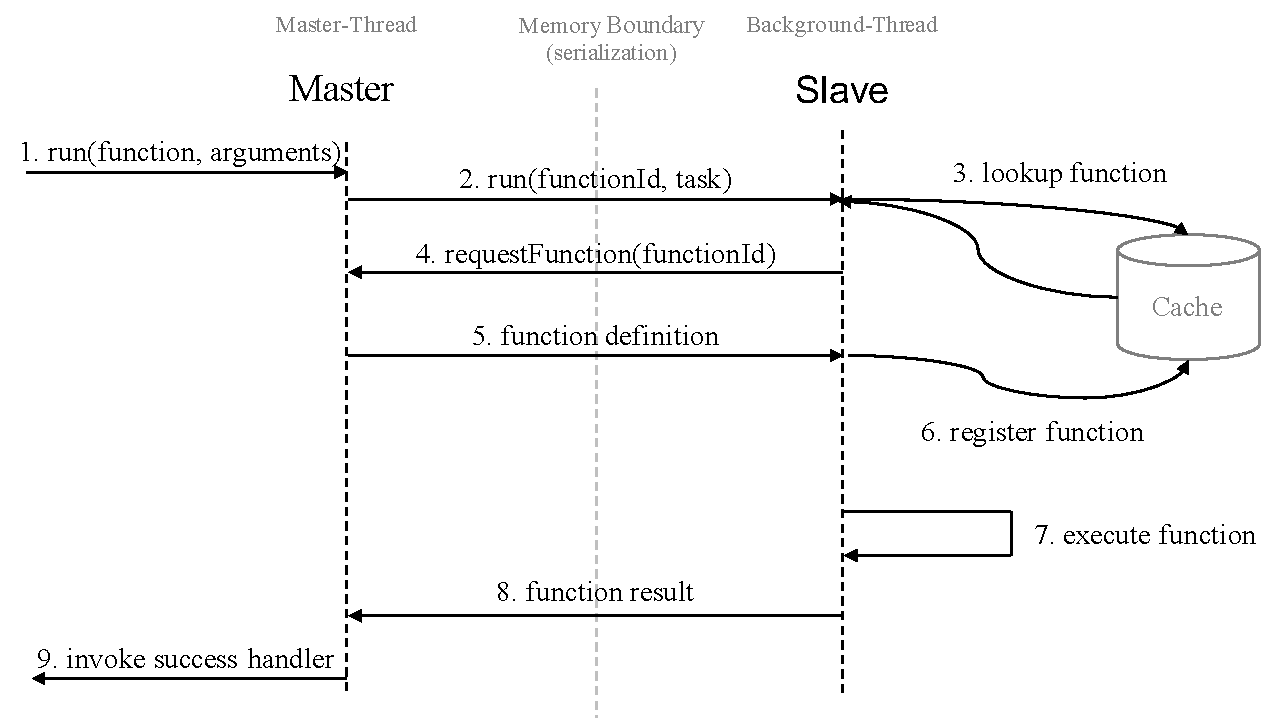
\includegraphics[width=0.8\textwidth]{runtime-system.pdf}

	\caption{Parallel.es Runtime System}
	\label{fig:runtime-system}
\end{figure*}

The caching of the function definitions on the slave have the advantage that performed JIT-optimizations are not thrown away if a task has completed. It is believed that the gain of reusing the JIT-Optimized function outweighs the additional costs caused by the function lookup and additional roundtrip for function retrieval. This especially for frequent but short running tasks for which the serialization overhead weights heavier. 


\subsection{Limitations}
The current implementation supports the essential features. However, it misses support for asynchronous task operations and the NodeJS environment. There are no technical reasons for not supporting either of these features. Adding support for NodeJS requires a structured clone polyfill to have the same behavior in NodeJS as in the browser.

A further limitation is that a task can not start other tasks. An efficient implementation to support recursive tasks requires a communication channel between all web workers that allows starting a task from a background thread on another, idle background thread without an additional roundtrip over the main thread. However, web workers only allow having a single communication channel between the thread that has started the Web Worker and the spawned web worker. Multiple channels are supported by Shared Workers that lack support in older browsers~\cite[section 4.6.4]{w3cWebWorker}.